\documentclass[runningheads]{llncs}
\usepackage[utf8]{inputenc}
\usepackage[T5]{fontenc}
\usepackage[vietnamese]{babel}
\usepackage{graphicx,booktabs,tabularx,array}
\usepackage[caption=false]{subfig}
\usepackage[hidelinks]{hyperref}
\graphicspath{{images/}}
\begin{document}
\title{Khảo sát bốn mô hình học máy cho bài toán phân loại hoa Iris}
\titlerunning{Khảo sát mô hình phân loại hoa Iris}
\author{Lê Văn Triệu\orcidID{0009-0002-3102-8391}}
\authorrunning{Lê Văn Triệu}
\institute{Trường Đại học Cần Thơ\\Học phần CT999 -- Công nghệ số nâng cao\\Mã số học viên M2526034\\\email{lvtrieu@ctu.edu.vn}}
\maketitle
\begin{abstract}
Bài viết khảo sát k láng giềng gần nhất, máy véc-tơ hỗ trợ, cây quyết định và rừng ngẫu nhiên trên dữ liệu Iris từ UCI. Mục đích là thực hành một quy trình có thể chạy lại, từ kiểm tra dữ liệu đến đối chiếu kết quả. Tệp gốc có 150 mẫu, bốn thuộc tính đo bằng cm và ba loài hoa. Sau khi loại ba dòng trùng hoàn toàn theo thuộc tính và nhãn, còn 147 mẫu. Dữ liệu được chia phân tầng thành 102 mẫu huấn luyện và 45 mẫu kiểm tra. Đánh giá chéo năm fold chỉ sử dụng tập huấn luyện. Trong lần chia với random\_state bằng 42, cây quyết định dự đoán đúng 42 trong 45 mẫu; ba mô hình còn lại đúng 41 mẫu. Kết quả cho thấy thứ tự theo F1 macro đánh giá chéo và theo tập kiểm tra có thể khác nhau. Quy mô dữ liệu nhỏ nên các chênh lệch được xem là kết quả của lần thực hành này.
\keywords{Iris \and Phân loại \and Đánh giá chéo \and Học máy}
\end{abstract}

\section{Giới thiệu}
Phân loại từ các số đo là một bài toán cơ bản của học máy có giám sát. Dữ liệu Iris gắn với nghiên cứu của Fisher~\cite{fisher} và hiện được UCI cung cấp công khai~\cite{iris}. Bốn đặc trưng có ý nghĩa cụ thể, vì vậy người học có thể xem trực tiếp các nhóm dữ liệu trước khi huấn luyện. Bài viết đặt câu hỏi: khi giữ cùng đầu vào và cùng cách chia dữ liệu, bốn mô hình cho kết quả như thế nào, và các lỗi nằm ở nhóm loài nào?

Các phương pháp được chọn có cách dự đoán khác nhau. kNN dựa trên các mẫu ở gần~\cite{cover}; SVM xây dựng ranh giới phân loại~\cite{cortes}; cây quyết định dùng các điều kiện trên thuộc tính~\cite{cart}. Random Forest kết hợp nhiều cây~\cite{breiman}, có liên hệ với cách lấy mẫu và kết hợp bộ dự đoán trong bagging~\cite{bagging}. Phạm vi khảo sát giới hạn ở một cấu hình cho mỗi mô hình. Bài viết không tìm tham số bằng kết quả trên tập kiểm tra.

\section{Dữ liệu và phương pháp}\label{sec:method}
\subsection{Nguồn và kiểm tra dữ liệu}
Sử dụng tệp \texttt{iris.data} trong gói tải từ UCI, sau đó thêm cột \texttt{source\_id} đánh số dòng và lưu thành CSV. Bốn thuộc tính gồm chiều dài, chiều rộng đài hoa và cánh hoa, cùng đơn vị cm. Nhãn gồm setosa, versicolor và virginica. Tệp CSV gốc được giữ riêng để đối chiếu. Bản dữ liệu này được xác định bằng tên tệp nguồn và mã băm trong dự án; kết quả không được gán cho một biến thể Iris khác.

Kiểm tra không phát hiện ô thiếu hoặc số đo không dương. Có ba dòng trùng hoàn toàn theo bốn đặc trưng cùng nhãn; giữ lần xuất hiện đầu tiên, lưu các dòng bị loại vào \texttt{dong\_trung.csv}. Đây là quy tắc xử lý của bài thực hành. Dữ liệu còn 147 dòng, gồm 48 setosa, 50 versicolor và 49 virginica. Việc loại trùng trước khi chia cũng tránh để các dòng giống hệt nhau xuất hiện ở cả hai tập. Hình~\ref{fig:scatter} cho thấy hai loài versicolor và virginica còn vùng chồng lấn khi chỉ xem hai thuộc tính cánh hoa.

\begin{figure}[t]
\centering
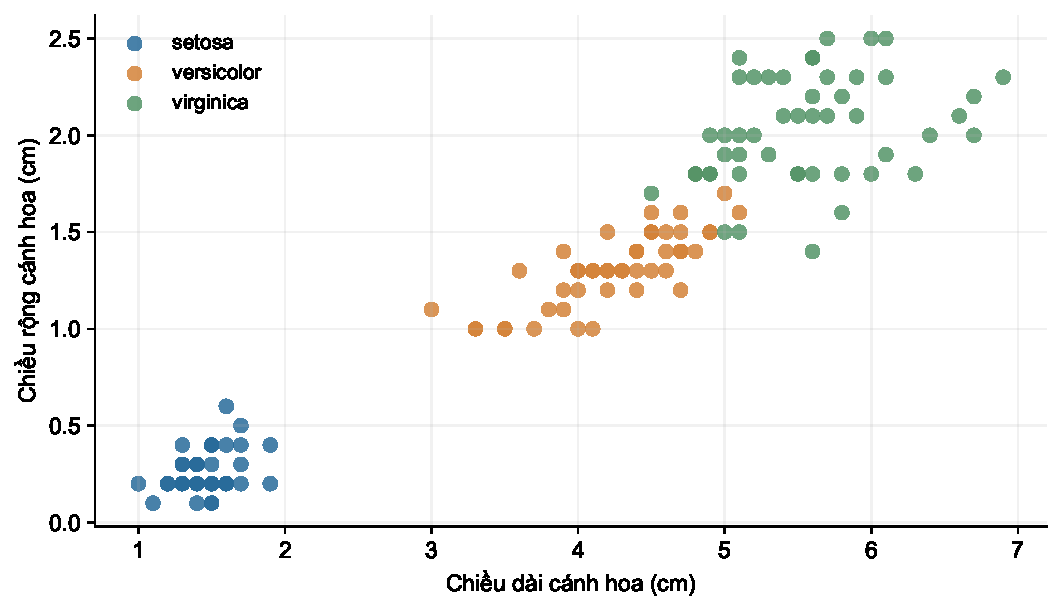
\includegraphics[width=.83\textwidth]{01_petal_scatter.pdf}
\caption{Chiều dài và chiều rộng cánh hoa trên 147 mẫu sau làm sạch. Các điểm trùng vị trí có thể che nhau.}\label{fig:scatter}
\end{figure}

\subsection{Chia dữ liệu và cấu hình mô hình}
Chia phân tầng 70\% cho huấn luyện và 30\% cho kiểm tra, với \texttt{random\_state=42}. Số mẫu thực tế là 102 và 45 do làm tròn. Tập kiểm tra có 15 mẫu mỗi loài. Dùng đánh giá chéo phân tầng năm fold trên 102 mẫu huấn luyện, có trộn với cùng hạt giống ngẫu nhiên. Cách dùng các phần dữ liệu để đánh giá được tham khảo từ nghiên cứu về đánh giá chéo~\cite{stone}.

kNN dùng \(k=5\). SVM dùng kernel RBF, \(C=1\) và \texttt{gamma=scale}. Hai mô hình này đặt \texttt{StandardScaler} trong \texttt{Pipeline}, để mỗi fold chỉ tính trung bình và độ lệch chuẩn từ phần huấn luyện của fold đó. Cây quyết định giới hạn độ sâu 3. Random Forest dùng 200 cây, hạt giống 42 và các tham số khác giữ mặc định của phiên bản thư viện đã lưu. Không áp dụng bộ chuẩn hóa cho hai mô hình cây.

\subsection{Thước đo và tệp đối chiếu}
Accuracy là tỷ lệ dự đoán đúng. F1 macro được tính theo Công thức~\ref{eq:f1}, trong đó \(P_c\) và \(R_c\) là precision và recall của lớp \(c\), \(K=3\). Mỗi loài đóng góp như nhau vào trung bình này.
\begin{equation}\label{eq:f1}
F1_{\mathrm{macro}}=\frac{1}{K}\sum_{c=1}^{K}\frac{2P_cR_c}{P_c+R_c}.
\end{equation}
Lưu giá trị F1 của từng fold, trung bình, độ lệch chuẩn mẫu, dự đoán từng dòng và ma trận nhầm lẫn. Nhờ \texttt{source\_id}, có thể tìm lại mẫu bị dự đoán sai trong CSV gốc. Phép tính và xử lý mảng sử dụng NumPy~\cite{numpy}; môi trường tính toán có SciPy~\cite{scipy}; các hình được vẽ bằng Matplotlib~\cite{matplotlib}. Phiên bản Python và thư viện được ghi trong \texttt{summary.json}.

\section{Kết quả và thảo luận}\label{sec:results}
\subsection{Kết quả đánh giá chéo và kiểm tra}
Bảng~\ref{tab:metrics} trình bày kết quả của cách chia ở Mục~\ref{sec:method}. Cột CV ghi trung bình cộng và độ lệch chuẩn mẫu trên năm fold. Cột test tính trên 45 mẫu đã tách riêng. Các giá trị được làm tròn bốn chữ số sau dấu thập phân khi trình bày; tệp CSV giữ độ chính xác cao hơn.
\begin{table}[t]
\caption{Kết quả chạy bốn mô hình. CV chỉ sử dụng tập huấn luyện.}\label{tab:metrics}
\centering\small
\begin{tabularx}{\textwidth}{l>{\centering\arraybackslash}X>{\centering\arraybackslash}X>{\centering\arraybackslash}X}
\toprule
Mô hình & F1 macro CV & Accuracy test & F1 macro test \\
\midrule
kNN & 0.9602 $\pm$ 0.0428 & 0.9111 & 0.9095 \\
SVM & 0.9597 $\pm$ 0.0667 & 0.9111 & 0.9107 \\
Decision Tree & 0.9501 $\pm$ 0.0628 & 0.9333 & 0.9327 \\
Random Forest & 0.9501 $\pm$ 0.0628 & 0.9111 & 0.9107 \\
\bottomrule
\end{tabularx}
\end{table}

kNN có F1 macro CV trung bình cao nhất, khoảng 0,9602. SVM đạt khoảng 0,9597, chênh lệch rất nhỏ so với kNN. Khi xem tập kiểm tra, cây quyết định đạt 42/45 dự đoán đúng, Accuracy khoảng 0,9333 và F1 macro khoảng 0,9327. Ba mô hình còn lại đúng 41/45 mẫu. kNN và SVM có cùng số dự đoán đúng nhưng F1 macro hơi khác nhau do lỗi phân bố khác nhau giữa các lớp.

\begin{figure}[t]
\centering
\subfloat[Số mẫu theo loài]{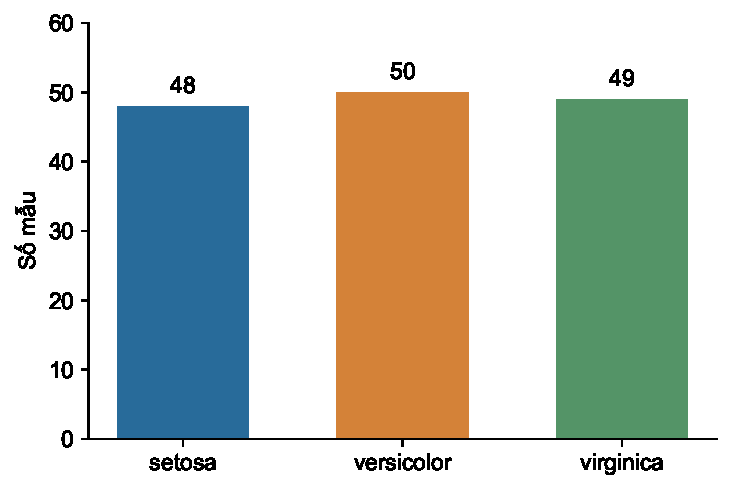
\includegraphics[width=.47\linewidth]{02_class_counts.pdf}}\hfill
\subfloat[Tương quan thuộc tính]{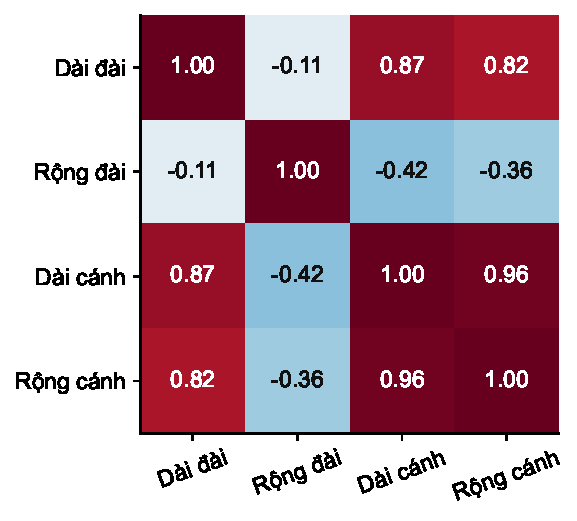
\includegraphics[width=.47\linewidth]{03_correlation.pdf}}\\
\subfloat[F1 macro CV và độ lệch chuẩn]{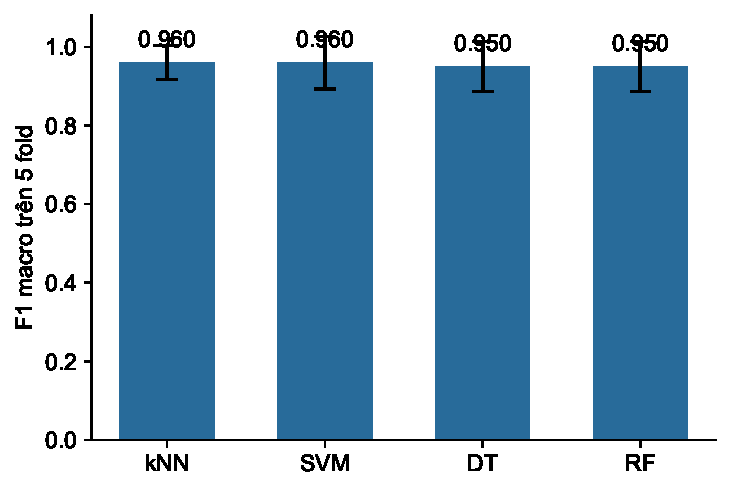
\includegraphics[width=.47\linewidth]{04_cv_f1.pdf}}\hfill
\subfloat[Ma trận nhầm lẫn SVM]{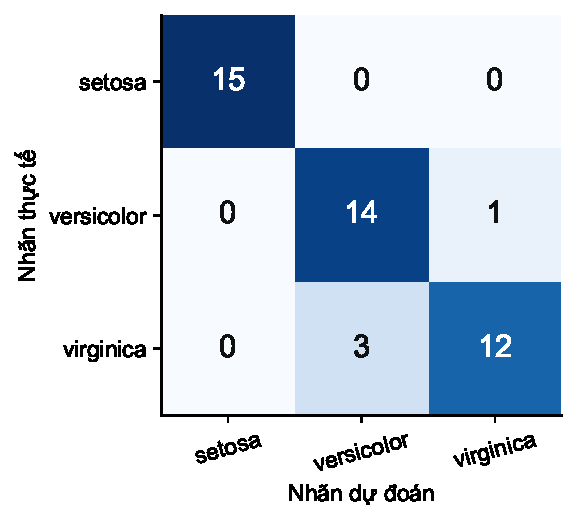
\includegraphics[width=.47\linewidth]{05_svm_confusion.pdf}}
\caption{Cụm bốn hình từ dữ liệu và kết quả chạy. Trong hình (d), hàng là nhãn thực tế, cột là nhãn dự đoán trên tập kiểm tra.}\label{fig:panels}
\end{figure}

\subsection{Quan sát lỗi và giới hạn}
Hình~\ref{fig:panels}(d) ghi nhận SVM phân loại đúng 15/15 mẫu setosa, 14/15 mẫu versicolor và 12/15 mẫu virginica. Một mẫu versicolor bị dự đoán thành virginica, còn ba mẫu virginica bị dự đoán thành versicolor. Điều này phù hợp với vùng chồng lấn quan sát ở Hình~\ref{fig:scatter}, nhưng hai thuộc tính được vẽ chưa mô tả toàn bộ không gian bốn chiều mà mô hình sử dụng.

Kết quả CV và test khác thứ tự không có nghĩa là một phép tính bị sai. Chúng sử dụng các mẫu đánh giá khác nhau và số lượng mẫu nhỏ. Chỉ một dự đoán đúng thêm đã làm Accuracy trên tập kiểm tra tăng khoảng 2,22 điểm phần trăm. Độ lệch chuẩn ở Hình~\ref{fig:panels}(c) cũng cho thấy kết quả thay đổi giữa các fold. Bài viết chưa kiểm định sự khác biệt giữa các mô hình và chưa khảo sát nhiều lần chia độc lập.

\section{Kết luận}
Quy trình đã đọc dữ liệu UCI, kiểm tra và loại dòng trùng theo quy tắc đã nêu, chia dữ liệu, huấn luyện bốn mô hình và lưu kết quả để chạy lại. Trong lần thực hành này, kNN có F1 macro CV trung bình cao nhất, còn cây quyết định có F1 macro test cao nhất. Các kết luận được giới hạn trong bộ dữ liệu và cấu hình đã sử dụng.

Hướng thực hiện tiếp là lặp lại đánh giá với các lần chia được xác định trước, thử một bộ dữ liệu lớn hơn và lựa chọn tham số chỉ trên phần huấn luyện. Dữ liệu, mã nguồn, dự đoán từng mẫu và các hình được lưu cùng bài nộp. Báo cáo này là bài thực hành khảo sát các phương pháp đã có.

\begin{thebibliography}{11}
\bibitem{fisher} FISHER, R.A.: The use of multiple measurements in taxonomic problems. Annals of Eugenics (1936). \doi{10.1111/j.1469-1809.1936.tb02137.x}.

\bibitem{cover} Cover, T., Hart, P.: Nearest neighbor pattern classification. IEEE Transactions on Information Theory (1967). \doi{10.1109/TIT.1967.1053964}.

\bibitem{cortes} Cortes, C., Vapnik, V.: Support-vector networks. Machine Learning (1995). \doi{10.1007/BF00994018}.

\bibitem{breiman} Breiman, L.: Random Forests. Machine Learning (2001). \doi{10.1023/A:1010933404324}.

\bibitem{bagging} Breiman, L.: Bagging predictors. Machine Learning (1996). \doi{10.1007/BF00058655}.

\bibitem{cart} Breiman, L., Friedman, J.H., Olshen, R.A., et al.: Classification And Regression Trees. Chapman and Hall/CRC (2017). \doi{10.1201/9781315139470}.

\bibitem{numpy} Harris, C.R., Millman, K.J., van der Walt, S.J., et al.: Array programming with NumPy. Nature (2020). \doi{10.1038/s41586-020-2649-2}.

\bibitem{scipy} Virtanen, P., Gommers, R., Oliphant, T.E., et al.: SciPy 1.0: fundamental algorithms for scientific computing in Python. Nature Methods (2020). \doi{10.1038/s41592-019-0686-2}.

\bibitem{matplotlib} Hunter, J.D.: Matplotlib: A 2D Graphics Environment. Computing in Science \& Engineering (2007). \doi{10.1109/MCSE.2007.55}.

\bibitem{stone} Stone, M.: Cross-Validatory Choice and Assessment of Statistical Predictions. Journal of the Royal Statistical Society Series B: Statistical Methodology (1974). \doi{10.1111/j.2517-6161.1974.tb00994.x}.

\bibitem{iris} Fisher, R.A.: Iris [Dataset]. UCI Machine Learning Repository (1936). \doi{10.24432/C56C76}.
\end{thebibliography}
\end{document}
